% Options for packages loaded elsewhere
\PassOptionsToPackage{unicode}{hyperref}
\PassOptionsToPackage{hyphens}{url}
%
\documentclass[
]{article}

\usepackage{amsmath,amssymb}
\usepackage{lmodern}
\usepackage{iftex}
\ifPDFTeX
  \usepackage[T1]{fontenc}
  \usepackage[utf8]{inputenc}
  \usepackage{textcomp} % provide euro and other symbols
\else % if luatex or xetex
  \usepackage{unicode-math}
  \defaultfontfeatures{Scale=MatchLowercase}
  \defaultfontfeatures[\rmfamily]{Ligatures=TeX,Scale=1}
\fi
% Use upquote if available, for straight quotes in verbatim environments
\IfFileExists{upquote.sty}{\usepackage{upquote}}{}
\IfFileExists{microtype.sty}{% use microtype if available
  \usepackage[]{microtype}
  \UseMicrotypeSet[protrusion]{basicmath} % disable protrusion for tt fonts
}{}
\makeatletter
\@ifundefined{KOMAClassName}{% if non-KOMA class
  \IfFileExists{parskip.sty}{%
    \usepackage{parskip}
  }{% else
    \setlength{\parindent}{0pt}
    \setlength{\parskip}{6pt plus 2pt minus 1pt}}
}{% if KOMA class
  \KOMAoptions{parskip=half}}
\makeatother
\usepackage{xcolor}
\usepackage[margin=1.5in]{geometry}
\usepackage{color}
\usepackage{fancyvrb}
\newcommand{\VerbBar}{|}
\newcommand{\VERB}{\Verb[commandchars=\\\{\}]}
\DefineVerbatimEnvironment{Highlighting}{Verbatim}{commandchars=\\\{\}}
% Add ',fontsize=\small' for more characters per line
\usepackage{framed}
\definecolor{shadecolor}{RGB}{248,248,248}
\newenvironment{Shaded}{\begin{snugshade}}{\end{snugshade}}
\newcommand{\AlertTok}[1]{\textcolor[rgb]{0.94,0.16,0.16}{#1}}
\newcommand{\AnnotationTok}[1]{\textcolor[rgb]{0.56,0.35,0.01}{\textbf{\textit{#1}}}}
\newcommand{\AttributeTok}[1]{\textcolor[rgb]{0.77,0.63,0.00}{#1}}
\newcommand{\BaseNTok}[1]{\textcolor[rgb]{0.00,0.00,0.81}{#1}}
\newcommand{\BuiltInTok}[1]{#1}
\newcommand{\CharTok}[1]{\textcolor[rgb]{0.31,0.60,0.02}{#1}}
\newcommand{\CommentTok}[1]{\textcolor[rgb]{0.56,0.35,0.01}{\textit{#1}}}
\newcommand{\CommentVarTok}[1]{\textcolor[rgb]{0.56,0.35,0.01}{\textbf{\textit{#1}}}}
\newcommand{\ConstantTok}[1]{\textcolor[rgb]{0.00,0.00,0.00}{#1}}
\newcommand{\ControlFlowTok}[1]{\textcolor[rgb]{0.13,0.29,0.53}{\textbf{#1}}}
\newcommand{\DataTypeTok}[1]{\textcolor[rgb]{0.13,0.29,0.53}{#1}}
\newcommand{\DecValTok}[1]{\textcolor[rgb]{0.00,0.00,0.81}{#1}}
\newcommand{\DocumentationTok}[1]{\textcolor[rgb]{0.56,0.35,0.01}{\textbf{\textit{#1}}}}
\newcommand{\ErrorTok}[1]{\textcolor[rgb]{0.64,0.00,0.00}{\textbf{#1}}}
\newcommand{\ExtensionTok}[1]{#1}
\newcommand{\FloatTok}[1]{\textcolor[rgb]{0.00,0.00,0.81}{#1}}
\newcommand{\FunctionTok}[1]{\textcolor[rgb]{0.00,0.00,0.00}{#1}}
\newcommand{\ImportTok}[1]{#1}
\newcommand{\InformationTok}[1]{\textcolor[rgb]{0.56,0.35,0.01}{\textbf{\textit{#1}}}}
\newcommand{\KeywordTok}[1]{\textcolor[rgb]{0.13,0.29,0.53}{\textbf{#1}}}
\newcommand{\NormalTok}[1]{#1}
\newcommand{\OperatorTok}[1]{\textcolor[rgb]{0.81,0.36,0.00}{\textbf{#1}}}
\newcommand{\OtherTok}[1]{\textcolor[rgb]{0.56,0.35,0.01}{#1}}
\newcommand{\PreprocessorTok}[1]{\textcolor[rgb]{0.56,0.35,0.01}{\textit{#1}}}
\newcommand{\RegionMarkerTok}[1]{#1}
\newcommand{\SpecialCharTok}[1]{\textcolor[rgb]{0.00,0.00,0.00}{#1}}
\newcommand{\SpecialStringTok}[1]{\textcolor[rgb]{0.31,0.60,0.02}{#1}}
\newcommand{\StringTok}[1]{\textcolor[rgb]{0.31,0.60,0.02}{#1}}
\newcommand{\VariableTok}[1]{\textcolor[rgb]{0.00,0.00,0.00}{#1}}
\newcommand{\VerbatimStringTok}[1]{\textcolor[rgb]{0.31,0.60,0.02}{#1}}
\newcommand{\WarningTok}[1]{\textcolor[rgb]{0.56,0.35,0.01}{\textbf{\textit{#1}}}}
\usepackage{longtable,booktabs,array}
\usepackage{calc} % for calculating minipage widths
% Correct order of tables after \paragraph or \subparagraph
\usepackage{etoolbox}
\makeatletter
\patchcmd\longtable{\par}{\if@noskipsec\mbox{}\fi\par}{}{}
\makeatother
% Allow footnotes in longtable head/foot
\IfFileExists{footnotehyper.sty}{\usepackage{footnotehyper}}{\usepackage{footnote}}
\makesavenoteenv{longtable}
\usepackage{graphicx}
\makeatletter
\def\maxwidth{\ifdim\Gin@nat@width>\linewidth\linewidth\else\Gin@nat@width\fi}
\def\maxheight{\ifdim\Gin@nat@height>\textheight\textheight\else\Gin@nat@height\fi}
\makeatother
% Scale images if necessary, so that they will not overflow the page
% margins by default, and it is still possible to overwrite the defaults
% using explicit options in \includegraphics[width, height, ...]{}
\setkeys{Gin}{width=\maxwidth,height=\maxheight,keepaspectratio}
% Set default figure placement to htbp
\makeatletter
\def\fps@figure{htbp}
\makeatother
\setlength{\emergencystretch}{3em} % prevent overfull lines
\providecommand{\tightlist}{%
  \setlength{\itemsep}{0pt}\setlength{\parskip}{0pt}}
\setcounter{secnumdepth}{5}
\usepackage{booktabs}

\usepackage{epsfig}
\usepackage{epstopdf}
\usepackage{rotate}
\usepackage{graphicx}
\usepackage{hyperref}
\usepackage{alphalph}
\usepackage{caption}
\usepackage[hang,flushmargin]{footmisc}
\usepackage{framed}
\usepackage{xcolor}
\usepackage{verbatim} 

\usepackage{bm}
\setcounter{MaxMatrixCols}{20}
\newcommand{\Var}{\mathrm{Var}}
\newcommand{\SD}{\mathrm{SD}}
\newcommand{\Cov}{\mathrm{Cov}}
\newcommand{\fx}{f({\bf x})}
\newcommand\R{{\textsf R~}}
\newcommand\Rst{\textsf{RStudio}}

% spacing between environments
\usepackage{amsthm}
\makeatletter
\def\thm@space@setup{%
  \thm@preskip=15pt plus 2pt minus 4pt
  \thm@postskip=\thm@preskip
}
\makeatother

% link colors in pdf?
\usepackage{xcolor}  
\definecolor{crimson}{RGB}{204,0,0}
\hypersetup{
  colorlinks = true,
  urlcolor = crimson,
  linkbordercolor = {white},
  linkcolor = crimson
}


% Title format
\usepackage{titling}
\pretitle{\Huge\sffamily}
\posttitle{\par\vskip 1em}
\predate{\LARGE\sffamily}
\postdate{\par}

\urlstyle{tt}
\ifLuaTeX
  \usepackage{selnolig}  % disable illegal ligatures
\fi
\usepackage[]{natbib}
\bibliographystyle{apalike}
\IfFileExists{bookmark.sty}{\usepackage{bookmark}}{\usepackage{hyperref}}
\IfFileExists{xurl.sty}{\usepackage{xurl}}{} % add URL line breaks if available
\urlstyle{same} % disable monospaced font for URLs
\hypersetup{
  pdftitle={Math Prefresher for Political Scientists},
  hidelinks,
  pdfcreator={LaTeX via pandoc}}

\title{Math Prefresher for Political Scientists}
\author{}
\date{\vspace{-2.5em}August 2023}

\usepackage{amsthm}
\newtheorem{theorem}{Theorem}[section]
\newtheorem{lemma}{Lemma}[section]
\newtheorem{corollary}{Corollary}[section]
\newtheorem{proposition}{Proposition}[section]
\newtheorem{conjecture}{Conjecture}[section]
\theoremstyle{definition}
\newtheorem{definition}{Definition}[section]
\theoremstyle{definition}
\newtheorem{example}{Example}[section]
\theoremstyle{definition}
\newtheorem{exercise}{Pencil Problem}[section]
\theoremstyle{definition}
\newtheorem{hypothesis}{Hypothesis}[section]
\theoremstyle{remark}
\newtheorem*{remark}{Remark}
\newtheorem*{solution}{Solution}
\newtheorem*{answer}{Answer}

\DeclareUnicodeCharacter{2212}{-}


\begin{document}

\setcounter{section}{1}

\section{Limits}

\begin{exercise}
\protect\hypertarget{exr:limseq2}{}\label{exr:limseq2}

Find the following limits of sequences, then explain in English the intuition for why that is the case.

\begin{enumerate}
\def\labelenumi{\arabic{enumi}.}
\tightlist
\item
  \(\lim\limits_{n\to\infty} \frac{2n}{n^2 + 1}\)
\item
  \(\lim\limits_{n\to\infty} (n^3 - 100n^2)\)
\end{enumerate}

\end{exercise}

\begin{solution}
\hfill
\begin{enumerate}
\item $0$. $n^2$ dominates $n$.
\item $\infty$. It just gets bigger.
\end{enumerate}
\end{solution}

\begin{exercise}[Limits of a Fraction of Functions]
\protect\hypertarget{exr:limfunmax}{}\label{exr:limfunmax}Find the limit of

\[\lim_{x\to\infty} \frac{(x^4 +3x−99)(2−x^5)}{(18x^7 +9x^6 −3x^2 −1)(x+1)}\]
\end{exercise}

\begin{solution}
Although this function seems large, the thing our eyes should focus on is where the highest order polynomial remains. That will grow the fastest, so if the highest order term is on the denominator, the fraction will converge to 0, if it is on the numerator it will converge to negative infinity. Previewing the multiplication by hand, we can see that the \(-x^9\) on the numerator will be the largest power. So the answer will be \(-\infty\). We can also confirm this by writing out fractions:

\begin{align*}  
& \lim_{x\to\infty}\frac{\left(1 + \frac{3}{x^3} - \frac{99}{4x^4}\right)\left(-\frac{2}{x^5} + 1\right)}{\left(1 + \frac{9}{18x} - \frac{3}{18x^5} - \frac{1}{18x^7} \right)\left(1 + \frac{1}{x}\right)} \\
&\times \frac{x^4}{1} \times -\frac{x^5}{1} \times \frac{1}{18x^7}\times \frac{1}{x}\\
=& 1 \times \lim_{-x\to\infty} \frac{x}{18}
\end{align*}
\end{solution}

Now, the functions will become a bit more complex:

\begin{exercise}
\protect\hypertarget{exr:discontlim}{}\label{exr:discontlim}

Solve the following limits of functions

\begin{enumerate}
\def\labelenumi{\arabic{enumi}.}
\tightlist
\item
  \(\lim\limits_{x\to 0} |x|\)
\item
  \(\lim\limits_{x\to 0} \left(1+\frac{1}{x^2}\right)\)
\end{enumerate}

\end{exercise}

\begin{solution}
\hfill
\begin{enumerate}
\item $0$
\item $\infty$
\end{enumerate}
\end{solution}

\begin{exercise}[Limit when Denominator converges to 0]
\protect\hypertarget{exr:discontdraw}{}\label{exr:discontdraw}

Let \[f(x) = \frac{x^2 + 2x}{x}.\]

\begin{enumerate}
\def\labelenumi{\arabic{enumi}.}
\tightlist
\item
  Graph the function. Is it defined everywhere?
\item
  What is the functions limit at \(x \rightarrow 0\)?
\end{enumerate}

\end{exercise}


\begin{solution}
See Figure \ref{fig:fig-hole-0}.

Divide each part by \(x\), and we get \(x + 2\) on the numerator, \(1\) on the denominator. So, without worrying about a function being not defined, we can say \(\lim_{x\to 0}f(x) = 0\).
\end{solution}

\begin{figure}
\centering
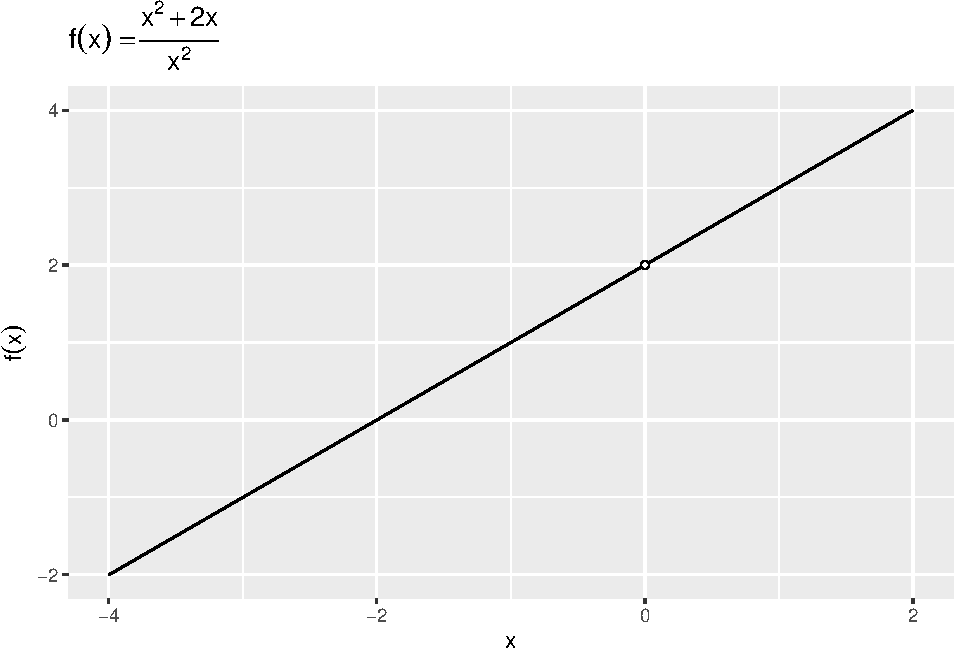
\includegraphics{figure-latex/fig-hole-0-1.pdf}
\caption{\label{fig:fig-hole-0}A function undedefined at x = 0}
\end{figure}

\newpage
\section{Derivatives}

\begin{exercise}[Derivative of Polynomials]
\protect\hypertarget{exr:introderivatives}{}\label{exr:introderivatives}

For each of the following functions, find the first-order derivative \(f^\prime(x)\).

\begin{enumerate}
\def\labelenumi{\arabic{enumi}.}
\tightlist
\item
  \(f(x)=c\)
\item
  \(f(x)=x\)
\item
  \(f(x)=x^2\)
\item
  \(f(x)=x^3\)
\item
  \(f(x)=\frac{1}{x^2}\)
\item
  \(f(x)=(x^3)(2x^4)\)
\item
  \(f(x) = x^4 - x^3 + x^2 - x + 1\)
\item
  \(f(x) = (x^2 + 1)(x^3 - 1)\)
\item
  \(f(x) = 3x^2 + 2x^{1/3}\)
\item
  \(f(x)=\frac{x^2+1}{x^2-1}\)
\end{enumerate}

\end{exercise}

\begin{solution}
\hfill
\begin{enumerate}
\def\labelenumi{\arabic{enumi}.}
\tightlist
\item
  \(f^\prime(x)= 0\)
\item
  \(f^\prime(x)= 1\)
\item
  \(f^\prime(x)= 2x^3\)
\item
  \(f\prime(x)= 3x^2\)
\item
  \(f\prime(x)= -2x^{-3}\)
\item
  \(f\prime(x)= 14x^6\)
\item
  \(f\prime(x) = 4x^3 - 3x^2 + 2x -1\)
\item
  \(f\prime(x) = 5x^4 + 3x^2 - 2x\)
\item
  \(f\prime(x) = 6x + \frac{2}{3}x^{\frac{-2}{3}}\)
\item
  \(f\prime(x)= \frac{-4x}{x^4 - 2x^2 + 1}\)
\end{enumerate}

\end{solution}

\begin{exercise}
\protect\hypertarget{exr:unnamed-chunk-19}{}\label{exr:unnamed-chunk-19}Let \(f(x,y)=x^3 y^4 +e^x -\log y\). What are the following partial derivaitves?
\begin{align*}
\frac{\partial f}{\partial x}(x,y) &=\\
\frac{\partial f}{\partial y}(x,y) &=\\
\frac{\partial^2 f}{\partial x^2}(x,y) &=\\
\frac{\partial^2 f}{\partial x \partial y}(x,y) &= 
\end{align*}
\end{exercise}

\begin{solution}
\hfill
\begin{enumerate}
\item $3x^2y^4 + e^x$
\item $4x^3y^3 - \frac{1}{y}$
\item $6xy^4 + e^x$
\item $12x^2y^3$
\end{enumerate}
\end{solution}

\end{document}
